	\documentclass{article}
\usepackage[utf8]{inputenc}
\usepackage{paralist}
\let\itemize\compactitem
\let\enditemize\endcompactitem
\let\enumerate\compactenum
\let\endenumerate\endcompactenum
\let\description\compactdesc
\let\enddescription\endcompactdesc

\usepackage{url}
\usepackage{enumerate}
\usepackage{graphicx}
\usepackage[a4paper,hmargin=0.75in,vmargin=1in]{geometry}
\usepackage{color}
\usepackage{enumerate}
\usepackage{subfigure}
\usepackage{graphicx}
\usepackage{comment}
\newtheorem{thm}{Theorem}
\usepackage{algorithm}
\usepackage{algorithmic}
\usepackage{float}
\usepackage{multirow}
\usepackage{setspace}
\usepackage{bigints}
\usepackage{booktabs}
\usepackage{hyperref}
\usepackage{amsfonts}
\usepackage{listings} %插入代码
\usepackage{xcolor} %代码高亮
\lstset{basicstyle=\footnotesize, %\tiny or \small or \footnotesize etc.
        numbers=left, %设置行号位置
        numberstyle=\tiny, %设置行号大小
        keywordstyle=\color{blue}, %设置关键字颜色
        commentstyle=\color[cmyk]{1,0,1,0}, %设置注释颜色
        frame=single, %设置边框格式
        escapeinside=``, %逃逸字符(1左面的键),用于显示中文
        breaklines, %自动折行
        extendedchars=false, %解决代码跨页时,章节标题,页眉等汉字不显示的问题
        xleftmargin=0.5em,xrightmargin=0.5em, aboveskip=0.1em, %设置边距
        tabsize=2, %设置tab空格数
        showspaces=false %不显示空格
       }

%Use Chinese
\usepackage[UTF8]{ctex}


\title{Word2Vec及BERT模型的水稻文献词汇嵌入计算}% Force line breaks with \\


\author{邓启东$^{1}$}

\date{
\textsuperscript{1}华中农业大学信息学院,430070,武汉,湖北,中国}



\begin{document}
\maketitle


\begin{abstract}

水稻由于其营养价值高,加工副产品用途广作为主要的粮食作物。有关水稻文献文本挖掘方面的研究十分重要。\par 本次课程论文在Pubmed文献数据库中以rice作为关键词获取6,859篇水稻文献摘要文本,并且利用经典的词嵌入方法Word2Vec的得到其中高频词的嵌入向量并进行t-SNE可视化以直观呈现水稻文献词汇间的相似性关系。并与BERT等方法进行比较。
最终凸显了BERT或Bio-BERT预先提供学习好的嵌入所带来的意义。

{\bf 关键词: 水稻, 词嵌入,t-SNE,Word2Vec}
\end{abstract}


\maketitle

\section{课题概况}
选修课程的目的主要在于我们生信的培养方案中涉及神经网络深度学习的内容较少。在学习了perl、R、python、shell等多种编程语言之后。而自然语言处理这门课程和生物信息学相结合,从生物文本中抽取知识,是学习一些比较智能的算法学习机会。在前面几次作业当中,我们发挥了充分的想象力进行下游分析。运用基础的代码进行了自主的探索。\par
选择嵌入计算的原因也在于Word2Vec算法本身设计的精妙。词语的向量分布式表示和神经网络的权重矩阵不谋而合。通过梯度下降逐渐找到一套合适的嵌入满足整个上下文文本。而且基于的是词语上下文相似则其语义相似的假设。相比于以往的各种方法而言是一大飞跃(在后文中也有所介绍)。可以使用相似性计算,取交叉熵的方式反映词汇之间的相似性。\par
本次课程论文计划能够很好的求出水稻文献中词汇的嵌入,并且通过t-SNE进行降维可视化。能够直观的感受到距离相近的词语的语义存在某种相似关联。就说明我们的算法是成功的。


\section{数据}

数据详见reference.table.txt,其搜集方式是通过在Pubmed上以rice作为关键词检索下载得到。\par
除去标题行共计6,859篇摘要,并且分为六列:标题、年份、期刊、发文机构、和基因(以``|''分隔)。\par
我们将其中的摘要抽取出来,将其中的特殊标点符号!"$\sharp$\$\%'()*+,./:;<=>?@[ $\backslash$]$\hat{}$\_`\{|\}$ \sim $全部替换成空格;并且将多个空格替换成一个空格,然后将单词全部转换成小写。把多个数字或者数字+字符+数字的组合替换成NBR。\par
至此,我们得到了以空格分开的每个单词构成的语料库,保存在data/corpus.txt路径下。
语料库数据准备完毕。
\section{研究方法}

\subsection{研究方法的算法背景,与其他方法的联系与区别}
在自然语言处理里面,最小的单位量是词语,词语组成句子,句子组成 段落,段落在组成一篇文章,所以在处理自然语言的问题时,首先要对最基本 的词语进行处理。\par
\subsubsection{词典}
我们想要表示一个词语,首先想到的是建立一个词典,而已经有这样一个词库WordNet\cite{2002Review}根据不同的词性建立起词和词的关系。实现词语分类,它是一种离散表征,反应不出词汇之间的差别。\par
这种方式存在以下两个弊端:
\begin{enumerate}

\item 缺少新词的含义;
\item 并不能完全的整合所有词,即便可以,它的数量也是十分庞大的。
\end{enumerate}
由于词语是符号形式的,计算机也无法理解,因此需要转换成数值形式。
\subsubsection{独热编码}
使用独热编码(one-hot)进行表示。 One-Hot 在特征提取上属于词袋模型(bag of words)。\par
 独热编码有明显的缺陷:
 \begin{enumerate}
\item 它不能表示所有的词,即从未出现过的合成词语
\item 无法表示和学习词语之间的相关性,反映不出文字天然的内在含义,每个词都是正交的,即所有的词语点积均为0,找不出相似词语
\item 会产生数据稀疏的问题,会浪费很多的存储空间
解决它的方法是利用派生词法(derivational morphology),也就是使用词根词缀的方式来避免一味增加词典的问题。但是派生词法本身也存在致命的问题,就是有的词根意义实在太多,重复的意思同样也会伤害词的表意。
\end{enumerate}
\subsubsection{矩阵分解}
通过SVD或者PCA降维等方式,将稀疏矩阵进行浓缩,得到一个低纬度稠密的类似矩阵。能更好的精炼词向量,并减少运算量。但是,这样的方法太过暴力,所得到的词向量效果也不好。

\subsubsection{语义分布表示(distributed representation)}
最早由Hinton提出,可以克服one-hot representation的上述缺点,基本思路是通过训练将每个词映射成一个固定长度的短向量,所有这些向量就构成一个词向量空间,每一个向量可视为该空间上的一个点。此时向量长度可以自由选择,与词典规模无关。这是非常大的优势。\par
自然语言处理最基本的单位就是词语。但是词语本身比如中文、英文都是符号形式的,如果想要构建数学模型,必须要转化为数值型的输入。或者说——嵌入到一个数学空间里,这种嵌入方式,就叫词嵌入(word embedding),而 Word2vec,就是词嵌入(word embedding) 的一种。\par
Word2Vec 是一种有效创建词嵌入的方法,它是从大量文本预料中以无监督方式学习语义知识的模型,这个模型为浅层双层的神经网络,用来训练以重新建构语言学之词文本。\par
Word2Vec 是轻量级的神经网络,其模型仅仅包括输入层,隐藏层和输出层,模型框架根据输入输出的不同,可以分为 CBOW 模型和 skip-gram 模型,CBOW 模型是通过上下文的内容预测中心词的可能情况,而 skip-gram 模型与其相反,它是通过中心词预测上下文词\cite{2013Efficient}。\par

\subsection{研究方法中的核心思路}
Skip-gram进行上下文预测的算法重点在于不断滑动改变中心词获得上下文最终生成批处理数据的过程。在这里我们使用“{\it 图 \ref{fig:example2}}”进行一个详细的展示,一些文献也对Skip-gram中的负采样有详细的描述\cite{2014word2vec}。\par
首先黑色框的部分是我们的语料库,并且由于我们已经有了一个独热编码的词语字典。因此语料库中的每一个词都可以转变为一个index。\par
下面蓝色的部分是一个buffer,它就像是一个纸带一样从整个语料库的左端向有段滑动。这里规定skip\_window(跳跃窗口)为4,也就是每个中心词单侧的词汇量。左右两边再加上中心词自身就是一个buffer的大小了,因而这里为9。
skip\_num是每次跳跃窗口选取训练模型词语,这里我们设置为8.实际上它一般小于两倍skip\_window,我们这里取等于,意味着中心词上下的8个词语全部抽出。并且储存到batch里。
\begin{figure}[H]
    \centering
    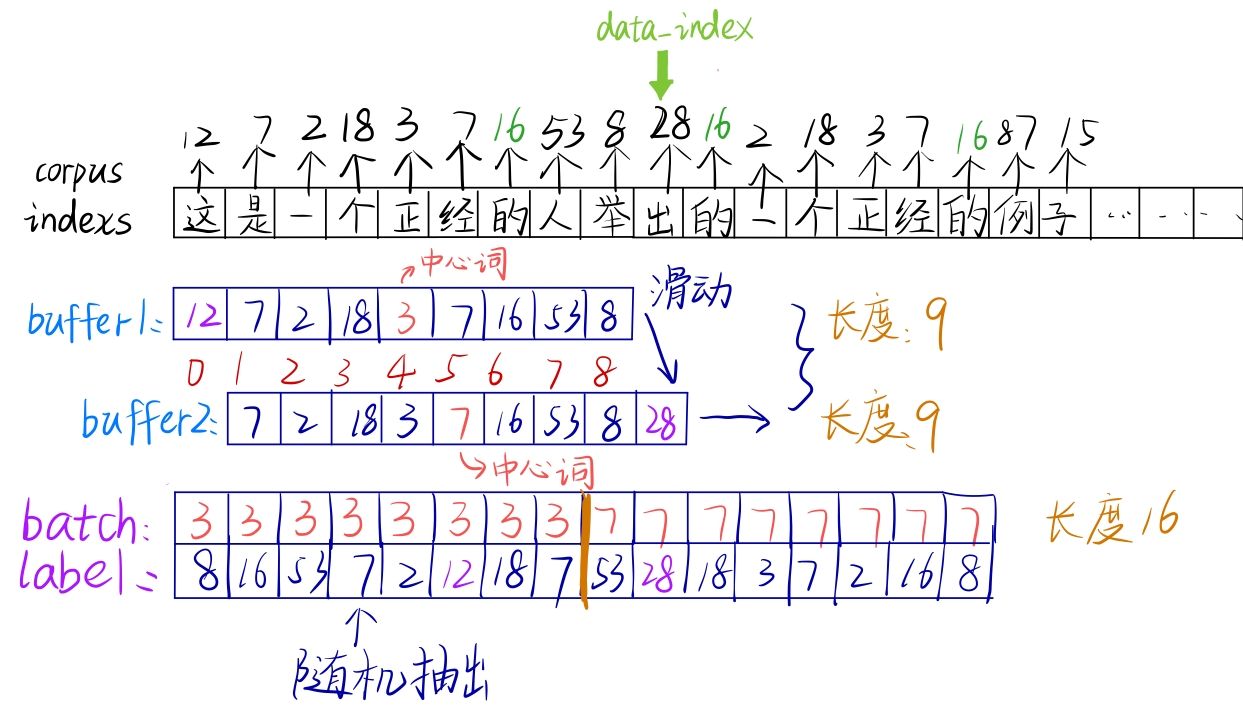
\includegraphics[width=0.7\textwidth]{figure/algorism.png}
    \caption{Skip-gram算法介绍。 图片来源:自绘\quad 工具:GoodNotes }
    \label{fig:example2}
\end{figure}


batch的3和7是中心词的index,下面的标签是抽出的上下文词汇。我们这里绘制的batch\_size是16,但是实际上在代码中是128。包括学习率在内,这些超参数均可以修改,而且会影响代码运行的时间和效果。

\subsection{本文的方法部分与课堂讲授内容的联系和区别/或补充}

本文其实和第七次实验最大的区别在于。我们拿到的语料库是直接的文本,需要自己先对其使用nltk包进行预处理。
\subsection{任务描述}

请详述本任务的主要设计,并解释所设计算法和代码能适应于此任务的原因。


\subsection{实验设计}
\subsubsection{语料库观察分析}
我们首先对语料库的title和abstract的字符数目进行一个统计(图\ref{zczxzx1})。其中(a)和(b)分别是这6,859篇摘要的标题和正文的长度频率分布直方图。其实整体可以看到存在为空的,尤其是abstract。但是最终我们都会把他们一起合并成语料库而且去掉其标点。所以去不去掉空的行对实验没有影响。
 \begin{figure}[H]
  \centering
  \subfigure[标题字符长度统计]{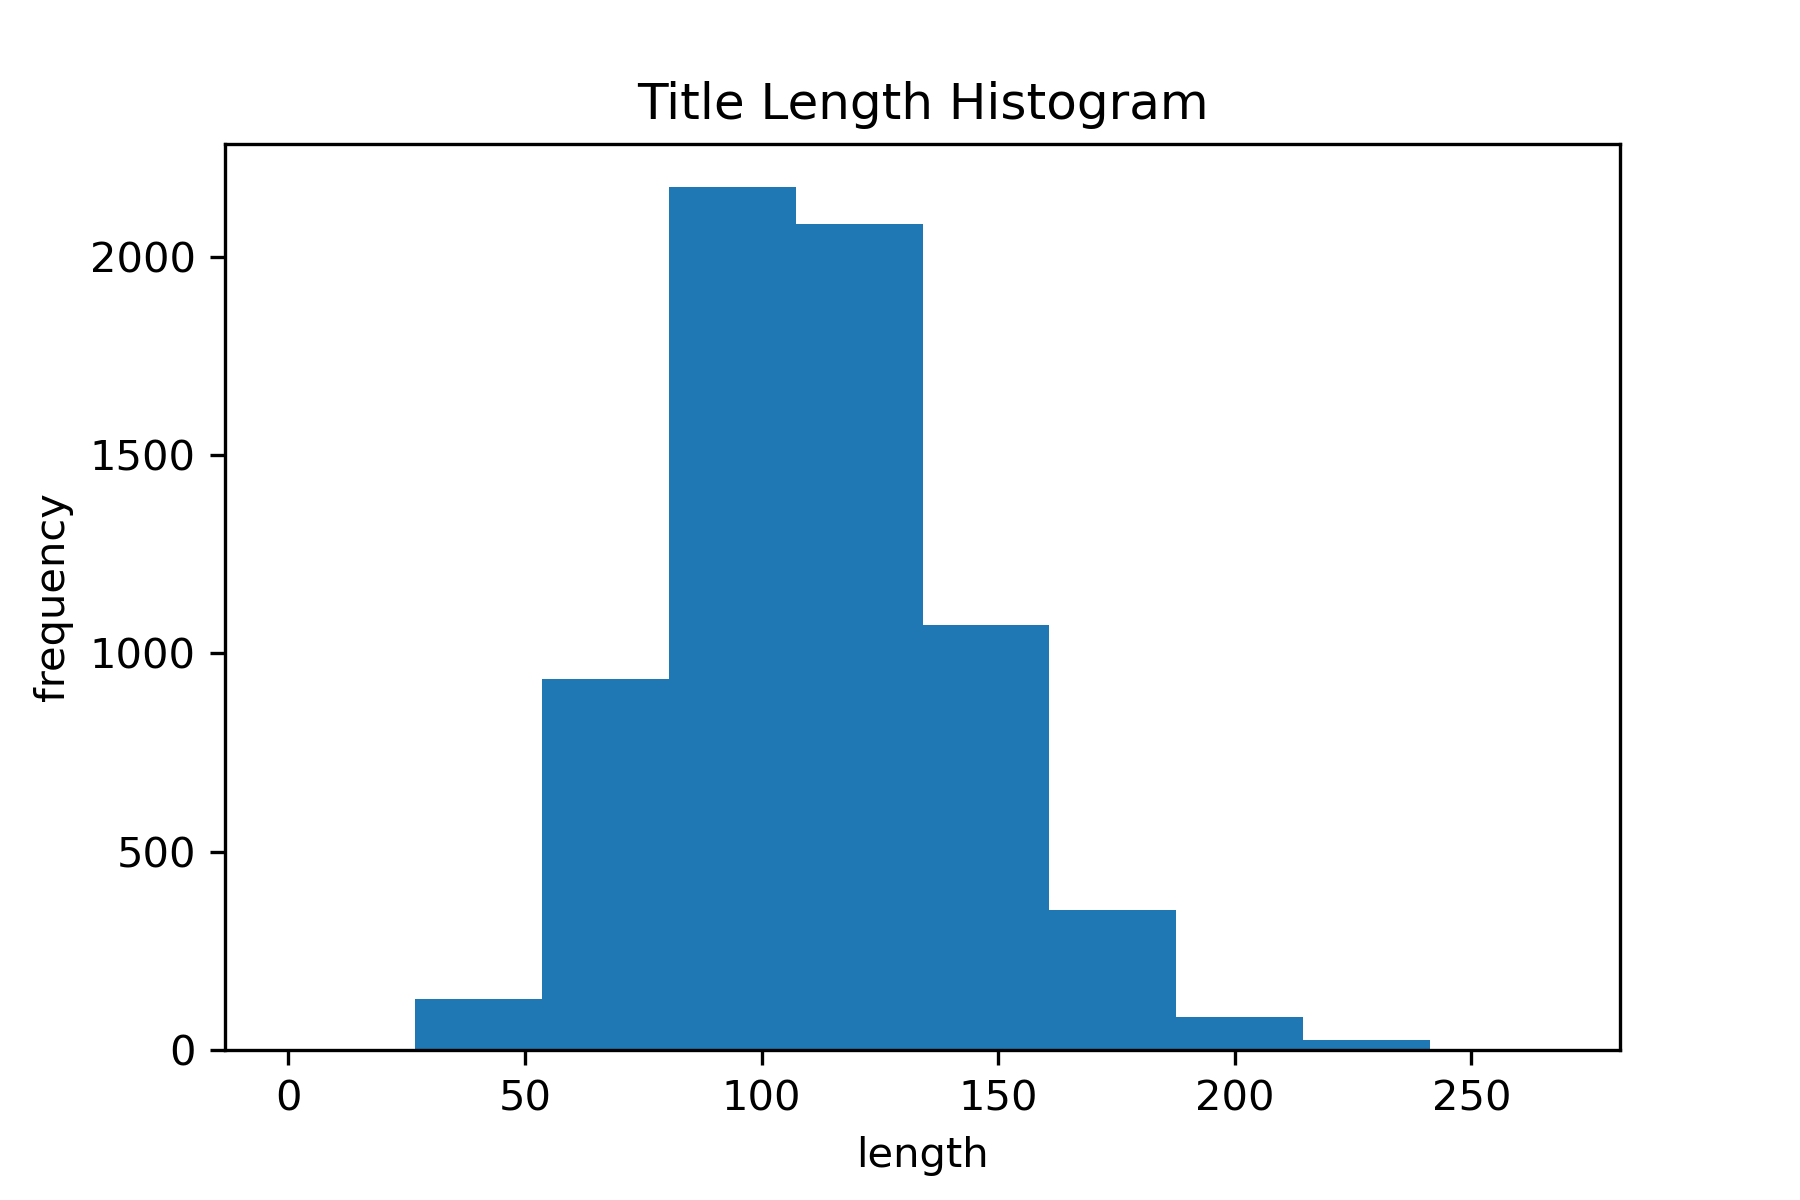
\includegraphics[width=3in]{figure/title.png}}
  \subfigure[摘要字符长度统计]{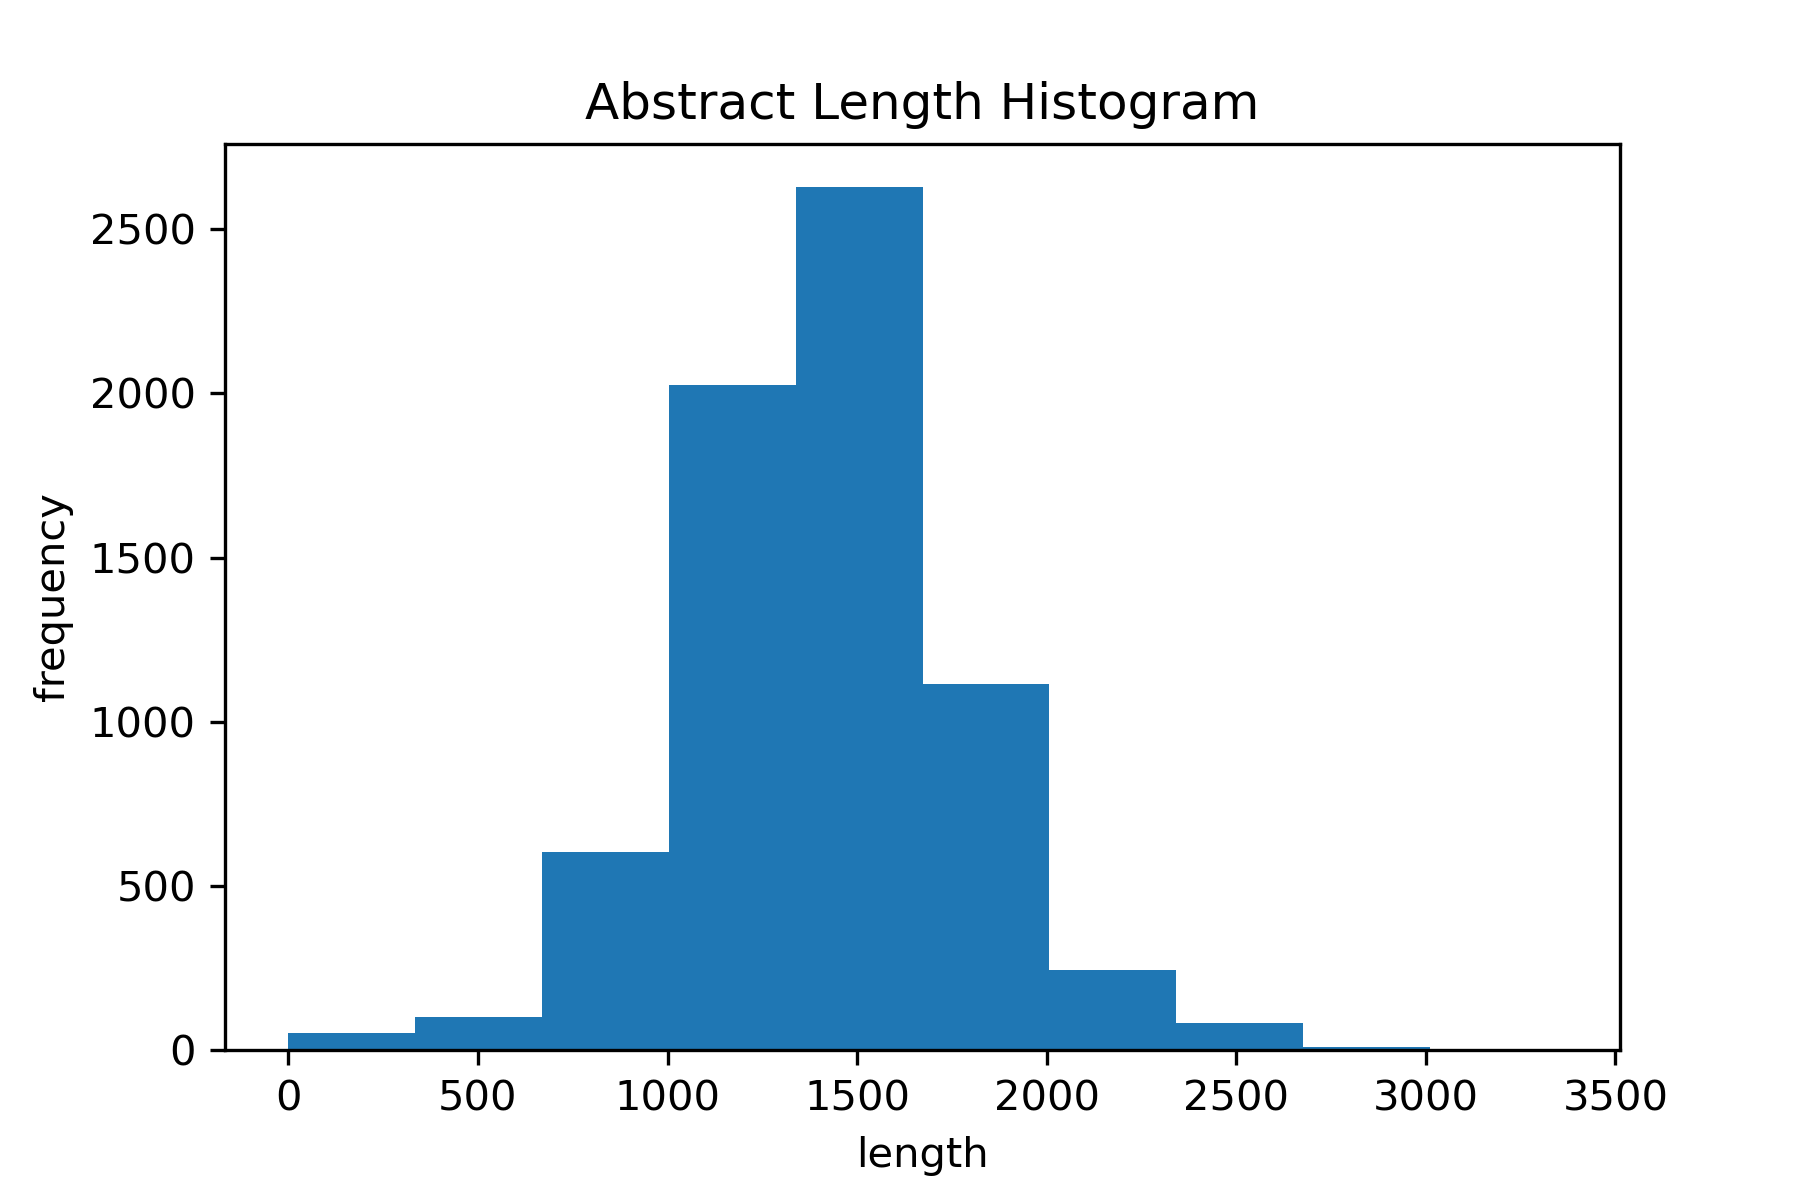
\includegraphics[width=3in]{figure/abstract2.png}}
  \caption{语料库字符长度统计}
  \label{zczxzx1}
\end{figure}

\subsection{某些关键代码}

\begin{lstlisting}[language=R]
代码来源:Tutorial_4_word2vec-main/Skip_Gram_basic.py第六步绘图
# Step 6: Visualize the embeddings.
def plot_with_labels(low_dim_embs, labels, filename='tsne.png'):
  assert low_dim_embs.shape[0] >= len(labels), "More labels than embeddings"
  print('Visualizing.')
  plt.figure(figsize=(18, 18))  #in inches
  for i, label in enumerate(labels):
    x, y = low_dim_embs[i,:]
    #if x< -25 or x>35 or y < -25 or y > 25:
        #continue
    plt.scatter(x, y)
    plt.annotate(label,
                 xy=(x, y),
                 xytext=(5, 2),
                 textcoords='offset points',
                 ha='right',
                 va='bottom')
  plt.savefig(filename)
  print('TSNE visualization is completed, saved in {0}.'.format(filename))
\end{lstlisting} 



\begin{figure}[H]
  \centering
  \subfigure[少数单词过滤前]{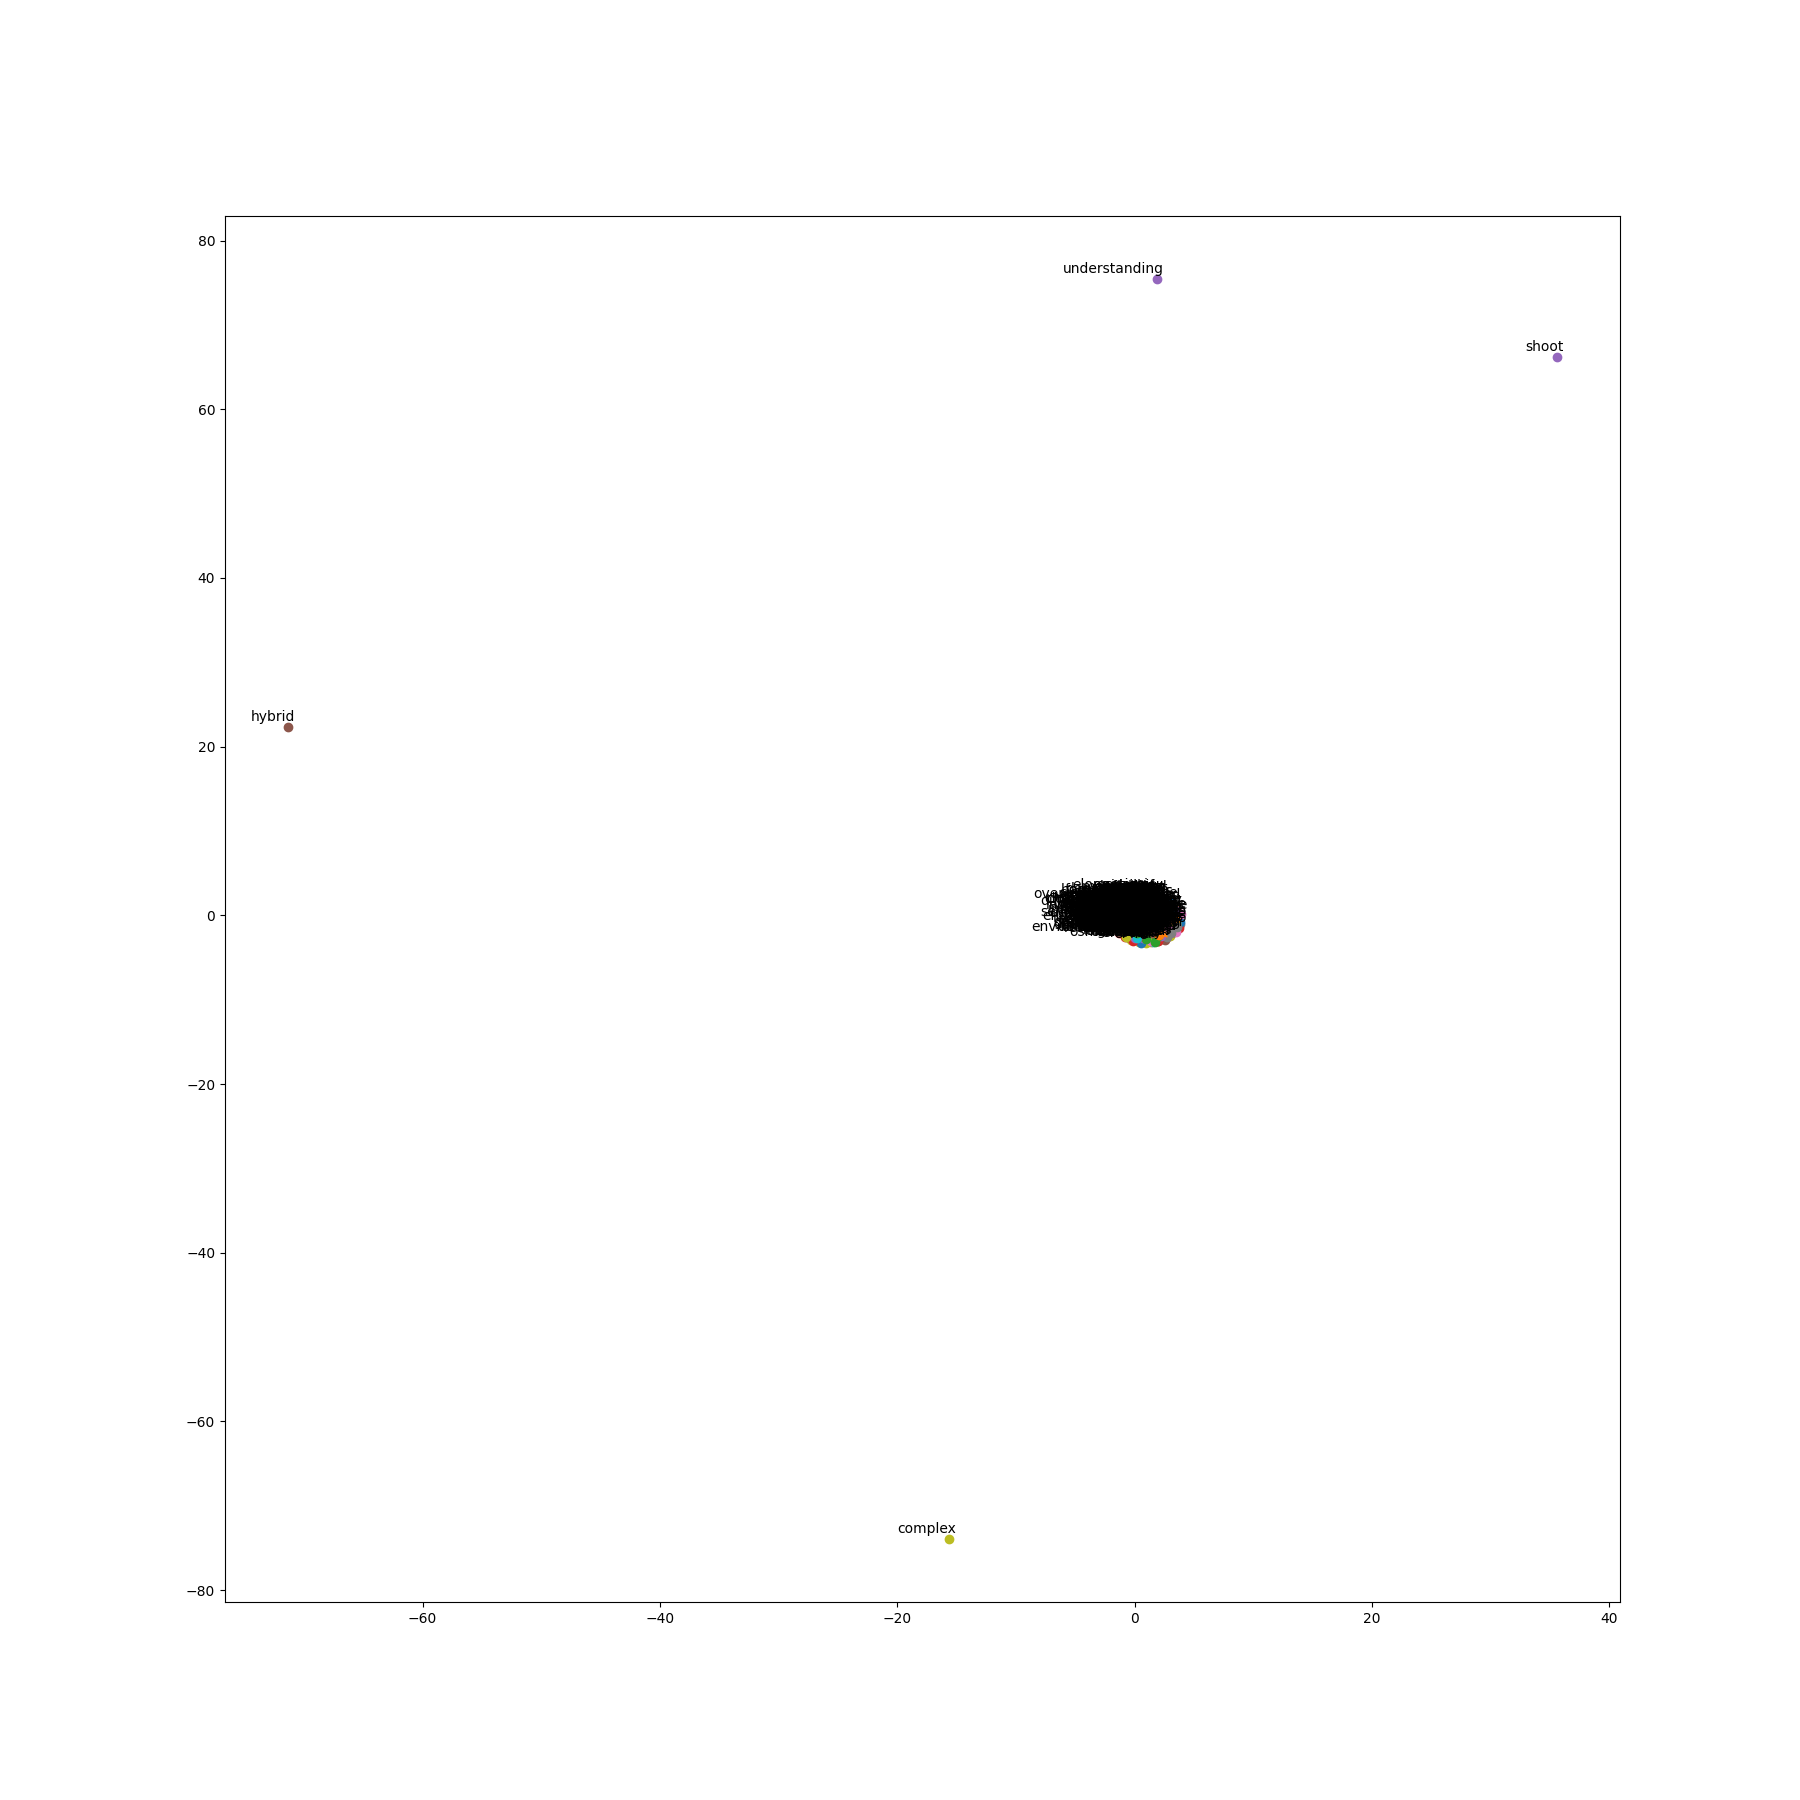
\includegraphics[width=3in]{figure/before.png}}
  \subfigure[控制坐标后]{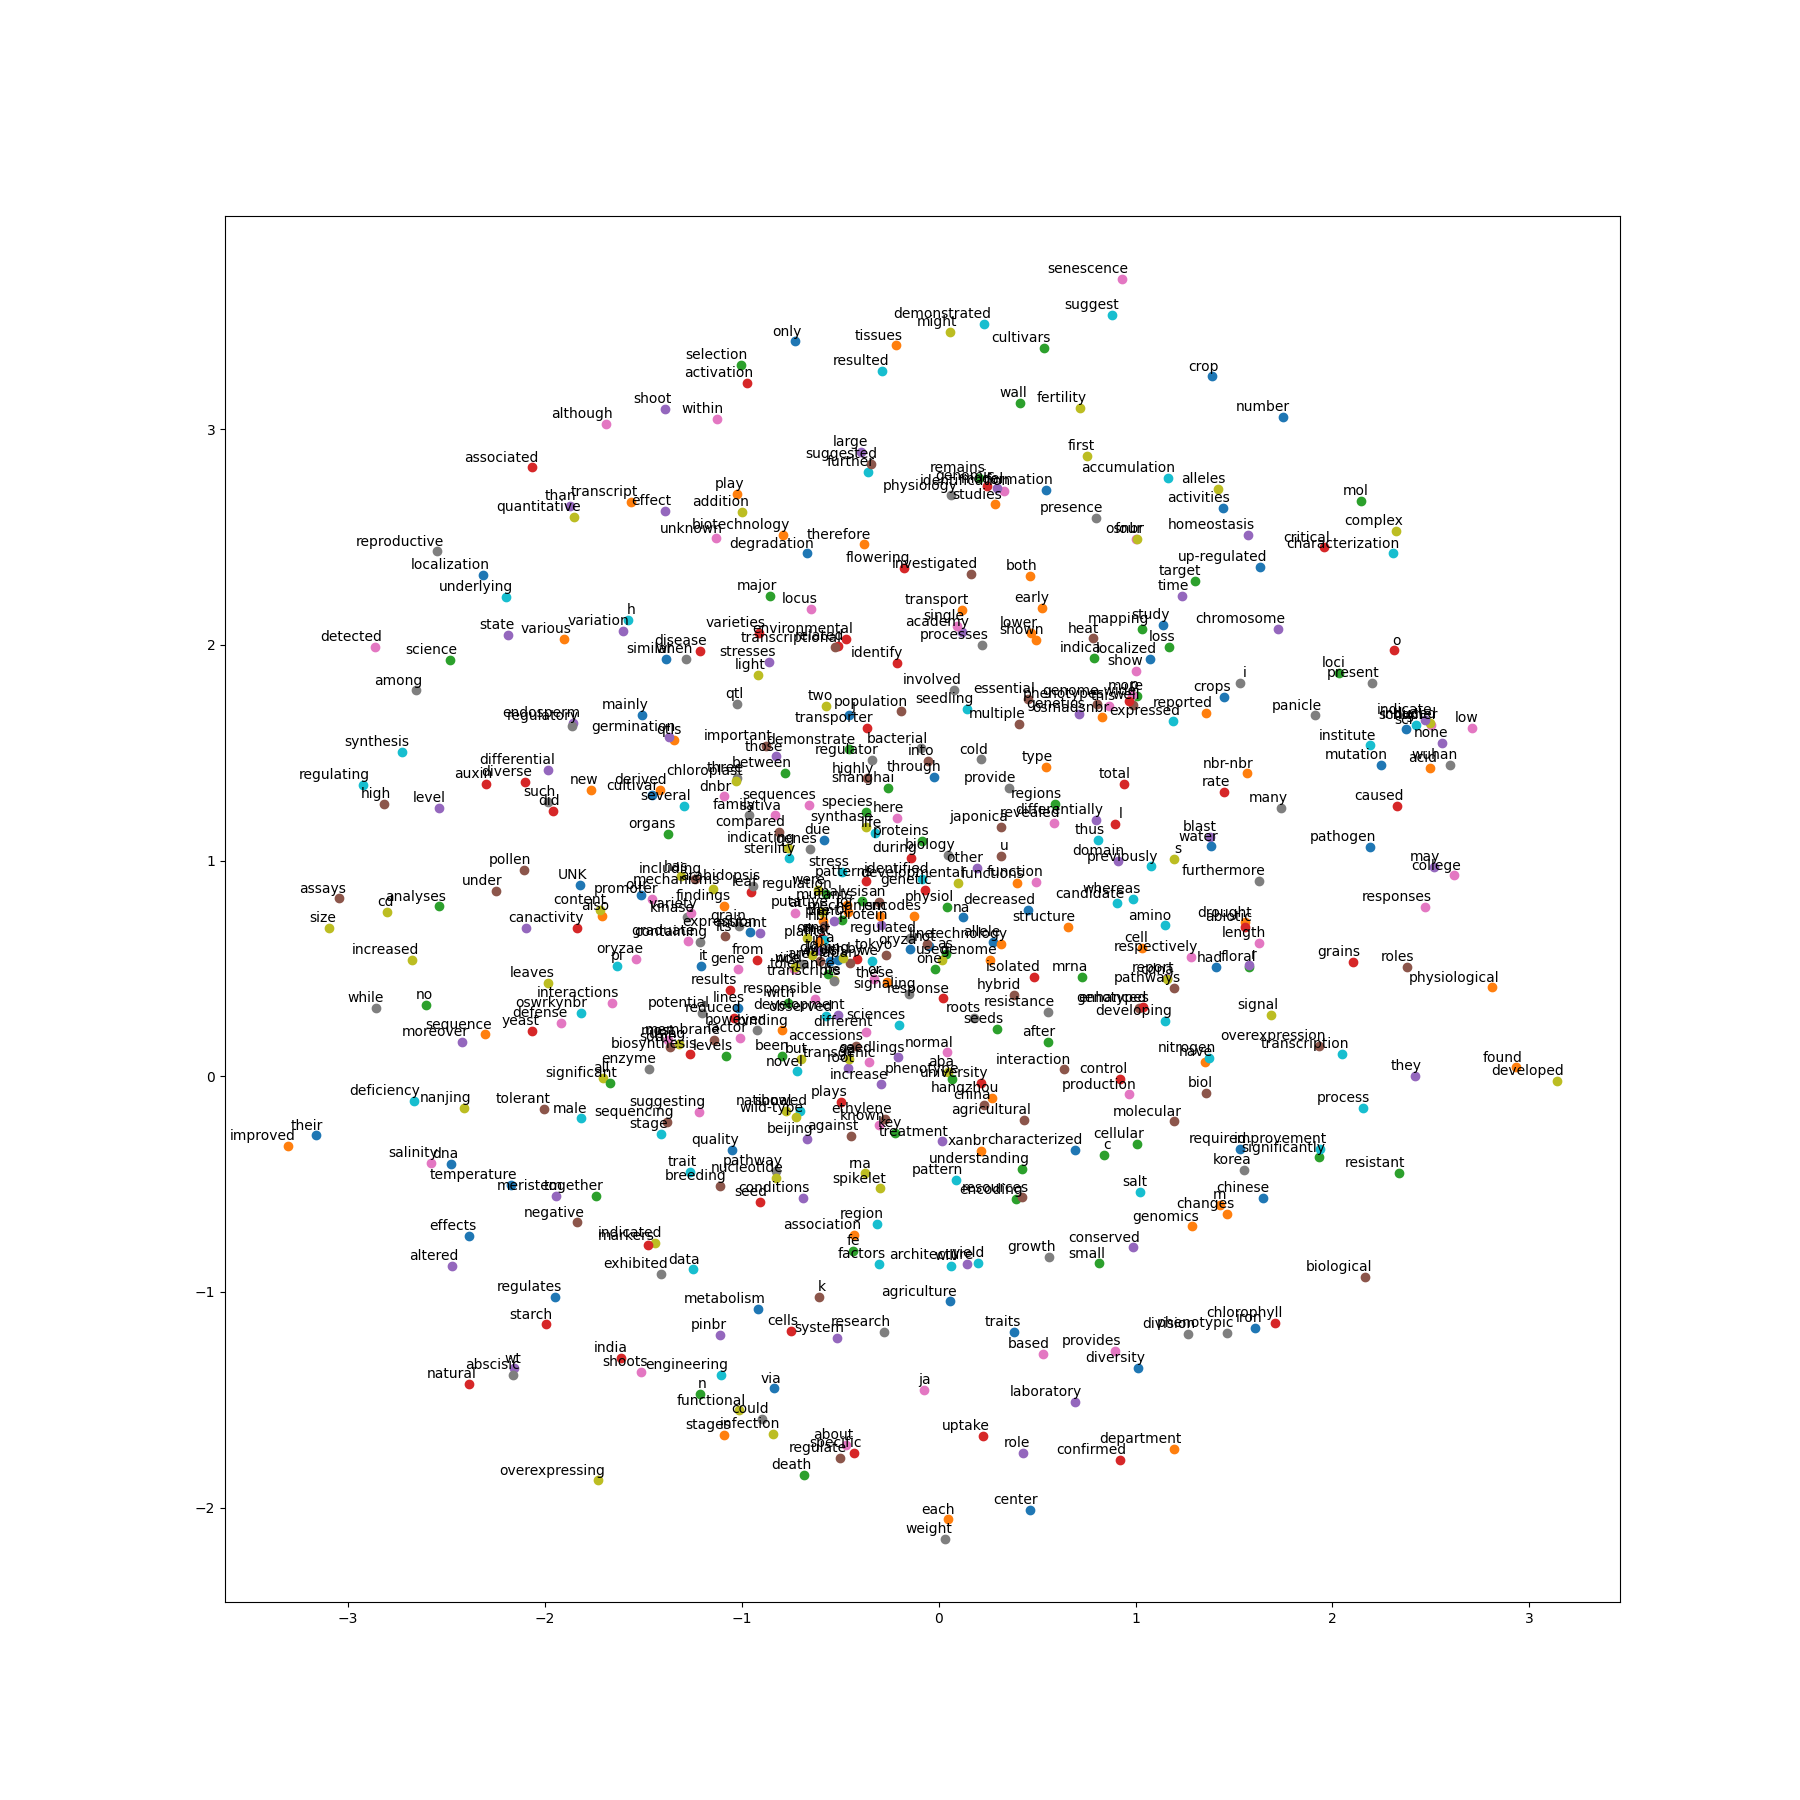
\includegraphics[width=3in]{figure/after.png}}
  \caption{t-SNE可视化结果}
  \label{zczxzx}
\end{figure}
分析这张图片(图\ref{zczxzx}(a))的坐标轴尺度为什么不太合适。我们看到原因是存在四个词语的嵌入非常的偏离大部分词语,他们分别是understanding、hybrid、shoot、complex,甚至达到了-70。原因是他们的上下文可能比较没有规律或者词频比较低。而其他的词语都在3上下。\par
比如当中绿色注释的两行通过限定x,y的范围都控制在25以内,如果超出countinue不参与绘图。以这样的方式过滤掉了比较偏离的那四个点。见图\ref{zczxzx}(b),t-SNE绘图的坐标轴变得合理了。
\section{\label{ch:experiment}主要的生物信息学实验和实验结论}
\subsection{结果分析}
我们从图中局部看到一些关联性。比如root和seed的距离就很近\par
此外还有salinity和temperature等环境因素。\par

本次实验的关联似乎没有第七次实验好,原因是训练的num\_steps只有1000,之后我们将其增加到8000,得到新的图片,不过区别不大,命名为tsne1.png

\section{\label{ch:postscript}后记}

2021年5月22日13时07,共和国勋章”获得者、中国工程院院士袁隆平老先生永远离开了我们。水稻作为我们亚洲的人口的主粮,袁隆平老先生培育的更加优秀的籼型杂交水稻对消除全世界人民的饥饿和贫困功不可没。就是这看似简单的一口饭,在过去的困苦年代是很难想象的。\par
见微知著,更加从这一次小的实验中体现出了BioNLP,或者说科研的意义。其实早在实体识别那一次作业就有涉及到水稻pubtator的实体识别,并且也发了一些有趣的联系。



\section{github}
\href{https://github.com/LianzePuppet/article}{\underline{github链接:}}https://github.com/LianzePuppet/article

\bibliographystyle{unsrt}
\bibliography{MyCitation}% Produces the bibliography via BibTeX.

\end{document}

\end{document}
